%%%%%%%%%%%%%%%%%%%%%%%%%%%%%%%%%%%%%%%%%%%%%%%%%%%
%
%  New template code for TAMU Theses and Dissertations starting Fall 2012.  
%  For more info about this template or the 
%  TAMU LaTeX User's Group, see http://www.howdy.me/.
%
%  Author: Wendy Lynn Turner 
%	 Version 1.0 
%  Last updated 8/5/2012
%
%%%%%%%%%%%%%%%%%%%%%%%%%%%%%%%%%%%%%%%%%%%%%%%%%%%
%%%%%%%%%%%%%%%%%%%%%%%%%%%%%%%%%%%%%%%%%%%%%%%%%%%%%%%%%%%%%%%%%%%%%%



\chapter{\uppercase{Iterative Acceleration for the $S_N$ Neutron Transport Equations}}
\label{sec:chapter4_acceleration}

Thus far, we have failed to discuss how the global system of angular flux unknowns is solved, 
focusing instead on the solution of a single system of equations that describes the unknowns of a single spatial cell, for a single discrete direction.
We have implicitly assumed the existence and knowledge of a transport sweep \cite{lewis_book}, or single, un-accelerated Richardson iteration.
In \secref{sec:dsa_basis}, we explain the fundamental iterative techniques used to solve the neutron transport equation for scatter media.
In \secref{sec:synthetics} we discuss the choices available for synthetic acclerators.
Finally  we two different synthetic acceleration techniques compatible with our chose spatial discretizations of the transport equation.
In \secref{sec:s2sa} we derive the $S_2$ synethetic acceleration (S2SA) technique\cite{s2sa} and in \secref{sec:dsa} we derive a modified interior penalty (MIP) diffusion synthetic accleration\cite{mip_dsa} (DSA) operator.  Finally, in \secref{sec:accel_results}, we compare verify the implementation of each for a set of test problems with spatially constant and and spatially varying interaction cross sections.


\section{Iterative Solution of the Neutron Transport $S_N$ Equations}
\label{sec:dsa_basis}

To describe the the iterative process by which the discrete ordinates neutron transport equations are solved, we re-visit the spatially analytic,
steady-state, mono-energetic discrete ordinates neutron transport equation, but do not have a monolithic right hand side source.
Rather, we treat the right hand side as having both an isotropic scattering component, and a fixed source component, as given in \eqt{eq:chap4_transport}.
\benum
\mu \frac{d \psi_d}{d x} + \Sigma_t \psi_d = \frac{\Sigma_s}{4\pi}\phi + S_d \pep
\label{eq:chap4_transport}
\eenum
The traditional practice is to solve \eqt{eq:chap4_transport} iteratively with Richardson iteration.  
Each Richardson iteration is referred to as a transport sweep, where for a fixed right hand side, $\psi_d$ is update direction by direction, cell be cell, sweeping 
from each direction's incident boundary through the entire mesh with upwinding at cell interfaces.
Introducing iteration index $\ell$, this process can be written as:
\benum
\mu \frac{d \psi_d^{(\ell+1)} }{d x} + \Sigma_t \psi_d^{(\ell+1)} = \frac{\Sigma_s}{4\pi}\phi^{(\ell)} + S_d \pep
\label{eq:chap4_iter}
\eenum
After we find, $\psi_d^{(\ell+1)}$, we update $\phi^{(\ell+1)}$ using the discrete ordinates definition:
\benum
\phi^{(\ell+1)} = 2\pi \sum_{d=1}^{N_{dir}}{w_d \psi_d^{(\ell+1)}} \pep
\eenum
Though convergent, the source iteration process can converge arbitrarily slow, as shown by Larsen\cite{larsen_dsa}, when $\frac{\Sigma_s}{\Sigma_t} \to 1$.
To accelerate the convergence of source iteration, the diffusion synthetic acceleration (DSA) technique was developed \cite{old_dsa}.
DSA is best explained through example.  

To start, we consider to a single source iteration:
\benum
\label{eq:chap4_iter1}
\mu \frac{d \psi_d^{(\ell+1/2)} }{d x} + \Sigma_t \psi_d^{(\ell+1/2)} = \frac{\Sigma_s}{4\pi}\phi^{(\ell)} + S_d \pep
\eenum
Subtracting \eqt{eq:chap4_transport} from \eqt{eq:chap4_iter1} yields:
\benum
\label{eq:chap4_err}
\mu \frac{d \delta \psi_d^{(\ell+1/2)} }{d x} + \Sigma_t \delta \psi_d^{(\ell+1/2)} = \frac{\Sigma_s}{4\pi} \delta \phi^{(\ell)} \pec
\eenum
where we have defined the iterative error of the angular flux, $\delta \psi_d^{(\ell+1)}$,
\benum
\psi_d = \psi_d^{(\ell+1)} + \delta \psi_d^{(\ell+1)} \pec
\eenum
and scalar flux iterative error, $\delta \phi^{(\ell)}$
\benum
\label{eq:chap4_phi_err}
\phi = \phi^{(\ell)} + \delta \phi_d^{(\ell)} \pep
\eenum
Subtracting $\frac{\Sigma_s}{4\pi} \delta \phi^{(\ell)}$ from both sides of \eqt{eq:chap4_err}, we see arrive at:
\benum
\mu \frac{d \delta \psi_d^{(\ell+1/2)} }{d x} + \Sigma_t \delta \psi_d^{(\ell+1/2)} - \frac{\Sigma_s}{4\pi} \delta \phi^{(\ell+1/2)}
= \frac{\Sigma_s}{4\pi} \delta \phi^{(\ell)} - \frac{\Sigma_s}{4\pi} \delta \phi^{(\ell+1/2)} \pep
\label{eq:chap4_intermediate}
\eenum
Recognizing:
\begin{subequations}
\beanum
\phi &=& \phi^{(\ell+1/2)} + \delta \phi^{(\ell+1/2)} \pec\\
\phi &=& \phi^{(\ell)} + \delta \phi^{(\ell)} \pec \\
\phi^{(\ell+1/2)} - \phi^{(\ell)} &=& \left( \phi - \delta \phi^{(\ell+1/2)}  \right) - \left( \phi -  \delta \phi^{(\ell)} \right) \pec \text{ and} \\
 \delta  \phi^{(\ell)} - \delta \phi^{(\ell+1)} &=& \phi^{(\ell+1/2)} - \phi^{(\ell)} \pec
\eeanum
\end{subequations}
\eqt{eq:chap4_intermediate} becomes:
\benum
\label{eq:dsa_idea}
\mu \frac{d \delta \psi_d^{(\ell+1/2)} }{d x} + \Sigma_t \delta \psi_d^{(\ell+1/2)} 
= \frac{\Sigma_s}{4\pi} \delta \phi^{(\ell+1/2)} + \frac{\Sigma_s}{4\pi} \left( \phi^{(\ell+1/2)} -  \phi^{(\ell)} \right) \pep
\eenum
Equation \ref{eq:dsa_idea} indicates that if we could solve a transport problem with a driving source equal to the difference between two scattering iterates,
\benum
\frac{\Sigma_s}{4\pi} \left( \phi^{(\ell+1/2)} - \phi^{(\ell)}  \right)\pec
\eenum
then we could get the iterative error of iteration $\delta \phi^{(\ell+1/2)}$, add to the $\phi^{(\ell+1/2)}$ we already have, and then have the exact solution, $\phi$. 
However, solving \eqt{eq:dsa_idea} is as difficult as solving the original problem in \eqt{eq:chap4_transport}.
Alternatively, if we could solve an approximation to \eqt{eq:dsa_idea}, perhaps the result would satisfy:
\benum
\label{eq:chap4_delta_phi}
\phi \approx \Delta \phi^{(\ell+1/2)} + \phi^{(\ell+1/2)} \pec
\eenum
where $\Delta \phi^{(\ell+1/2)}$ comes from the lower order approximation to \eqt{eq:dsa_idea}.
The idea of a using lower order approximation to approximately solve \eqt{eq:dsa_idea} is central to synthetic acceleration.


\section{Qualitative Comparison of Different Synthetic Acceleration Techniques}
\label{sec:synthetics}

Three types of synthetic acceleration have received significant attention in the neutron transport and thermal radiative transfer literature,
$S_2$ synthetic acceleration (S2SA)\cite{s2sa}, diffusion synthetic acceleration (DSA)\cite{old_dsa}, and transport synthetic acceleration (TSA)\cite{tsa}.
Each method of synthetic acceleration has both advantages and disadvantages relating to the computational efficiency and iterative effectiveness of each method.  

The S2SA method was shown to be iteratively effective in both slab and 1-D spherical geometries. 
Additionally, it is easily compatible with any DFEM spatial discretization of the $S_N$ neutron transport equations.  
S2SA solves for $\psi_+$ and $\psi_-$ using a single global matrix solve, rather than a direction by direction solve for the full transport $\psi_d$ unknowns.
The full transport scalar flux iterative update is then defined as,
\benum
\Delta \phi^{(\ell+1/2)} \approx 2\pi \left[ w_+ \psi_+ + w_- \psi_- \right] \pec
\eenum
where $w_+,~w_-$ correspond to the weights of a direction quadrature (typically Gauss) set with corresponding discrete direction $\mu_+ and \mu_-$, and $\psi_+,~\psi_-$ are the fundamental unknowns of the $S_2$ discretization.
Thus, S2SA uses the same local matrices of \eqt{eq:chap3_mat_form} as the full transport operator.
However, the S2SA global matrix that must be inverted to solve for $\psi_+$ and $\psi_-$ is extremely difficult to invert for multiple spatial dimensions.
This makes S2SA iteratively effective, but computationally expensive, limiting the extensibility of any techniques that require S2SA.
But since our initial focus is on solving slab geometry neutron transport problems, we will continue to consider S2SA as it is readily adaptable to our new spatial discretization schemes. \cite{s2sa}

Gelbard and Hageman first showed in \cite{old_dsa} that diffusion synthetic acceleration (DSA) could be used to accelerate the convergence of source iteration in neutron transport since the diffusion operator effectively attenuates the slowly varying error modes that hinder the convergence of source iteration.
To be unconditionally effective, Larsen showed that DSA needed to be derived in a method consistent with the spatial and angular discretization of the transport equation \cite{larsen_dsa}.
Adams and Martin first showed that partially consistent diffusion discretizations could be used to effectively accelerate DFEM spatial discretizations of the neutron transport equation \cite{adams_dsa}.
Though shown to be unconditionally stable for certain geometries the M4S DSA proposed in \cite{adams_dsa} has been shown to be unstable for unstructured multi-dimensional geometries \cite{wwm_dsa}.
To allow more general applicability, we wish to consider a more advanced DSA discretization.
Alternative DSA discretizations that have been applied successfully to unstructured multi-dimensional geometries include: the partially consistent WLA DSA proposed in \cite{wla_dsa}, the fully consistent DSA (FCDSA) proposed in \cite{wwm_dsa}, and the partially consistent MIP DSA proposed in \cite{mip_dsa}.
WLA DSA produces a symmetric positive definite (SPD) diffusion matrix and is unconditionally stable, but the spectral radius of the WLA DSA scheme increases on distorted mesh cells and for optically thick cells with scattering ratios very close to unity \cite{wla_dsa,wwm_dsa}.
While the FCDSA scheme remains effective in optically thick cells, it creates a diffusion operator that is very difficult and costly to invert\cite{wwm_dsa}. 
The MIP DSA discretization \cite{mip_dsa} of Wang and Ragusa generates a SPD diffusion operator, remains effective for all cell optical thicknesses, has been successfully applied to high order DFEM $S_N$ transport, and can be used with adaptive mesh refinement.
Further, it was shown in \cite{mip_mc} that the MIP DSA diffusion operator can be inverted very quickly using advanced preconditioners such as algebraic multi-grid.
Thus, it we can ideally define a MIP discretization that is iteratively effective for neutron transport problems discretized with our higher order DFEM methods that account for the spatial variation of cross section within each cell, we will have found a scheme that is most likely to prove useful in more meaningful (multiple spatial dimension) thermal radiative transfer simulations.

 TSA differs from S2SA and DSA in that it does not attempt to invert a single matrix that describes a lower order operator approximation to the full discrete ordinates neutron transport equation.
The main advantage of TSA over DSA is that using TSA allows for re-use of much of the software already developed for transport sweeps, greatly lowering software development overhead as compared to using DSA.
However, TSA is in general not as effective as DSA, and finding the most efficient set of parameters that complete the description of the TSA scheme is problem dependent.  \cite{tsa}

We will derive an S2SA operator in \secref{sec:s2sa} and MIP DSA operator in \secref{sec:dsa}.  
We elect not to derive a TSA operator as it occupies a middle ground between, a S2SA operator that re-uses a lot of the transport sweep capability we have already developed with our high order DFEM of Chapter \ref{sec:chapter3_variable_xs}, but is computationally challenging to invert (in multiple spatial dimensions), and the MIP DSA operator we define in \secref{sec:dsa} that requires significant derivation independent of the DFEM neutron transport methodology we have already derived, but that is computationally efficient to invert.

\section{$S_2$ Synthetic Acceleration}
\label{sec:s2sa}

We begin our derivation by repeating the $S_2$, spatially analytic angular flux update equations from Morel\cite{s2sa} (Eqs. (12a) and (12b)), noting that we have elected to use $\psi^+$ and $\psi^-$ instead of $c^+$ and $c^-$, $\Sigma$ represents macroscopic interaction cross sections rather than $\sigma$,  and we define $\phi = 2\pi \sum_d{w_d \psi_d}$:
\begin{subequations}
\label{eq:chap4_raw}
\benum
\mu_+ \frac{d \psi^+}{dx} + \Sigma_t \psi^+ = \frac{\Sigma_s}{4\pi} \Delta \phi + \frac{\Sigma_s}{4\pi} \left( \phi^{(\ell+1/2)} - \phi^{(\ell)} \right) 
\eenum
\benum
\mu_- \frac{d \psi^-}{dx} + \Sigma_t \psi^- = \frac{\Sigma_s}{4\pi}{\Delta \phi} + \frac{\Sigma_s}{4\pi} \left( \phi^{(\ell+1/2)} - \phi^{(\ell)} \right) \pep
\eenum
\end{subequations}
In \eqts{eq:chap4_raw} we are assuming scattering is isotropic only.
Spatially discretizing with a $P$ degree DFEM as in Chapter \ref{sec:chapter3_variable_xs}, for an interior cell, $c$, we  have:
\begin{subequations}
\label{eq:chap4_first_disc}
\benum
\left( \mu_+ \mathbf{G}_+ + \frac{\Delta x_c}{2}\mathbf{R}_{\Sigma_t}\right) \vec{\psi}^+_c = \frac{\Delta x_c}{8\pi} \mathbf{R}_{\Sigma_s} \vec{\Delta \phi}_c
+ \frac{\Delta x_c}{8\pi} \mathbf{R}_{\Sigma_s} \left( \vec{\phi}_c^{(\ell+1/2)} - \vec{\phi}_c^{(\ell)} \right) + \mu_+ \psi_{in,+} \vec{f}_+ 
\eenum
\benum
\left( \mu_- \mathbf{G}_- + \frac{\Delta x_c}{2}\mathbf{R}_{\Sigma_t}\right) \vec{\psi}^-_c = \frac{\Delta x_c}{8\pi} \mathbf{R}_{\Sigma_s} \vec{\Delta \phi}_c 
+ \frac{\Delta x_c}{8\pi} \mathbf{R}_{\Sigma_s} \left( \vec{\phi}_c^{(\ell+1/2)} - \vec{\phi}_c^{(\ell)} \right) + \mu_- \psi_{in,-} \vec{f}_-  \pep
\eenum
\end{subequations}
In \eqts{eq:chap4_first_disc}, we note that $\mu_+ > 0$ and $\mu_- < 0$, and as such use the $\pm$ subscripts to define the appropriate $\mathbf{G}$ and $\vec{f}$, defined in \eqts{eq:chap4_g} and \eqts{eq:chap4_f}, respectively:
\begin{subequations}
\label{eq:chap4_g}
\benum
\mathbf{G}_{+,i~j} = \B{i}(1)\B{j}(1) - \int_{-1}^1{\frac{ d \B{i}}{d s} \B{j}(s) ~ds}
\eenum
\benum
\mathbf{G}_{-,i~j} = -\B{i}(-1)\B{j}(-1) - \int_{-1}^1{\frac{ d \B{i}}{d s} \B{j}(s) ~ds} \pec
\eenum
\end{subequations}
\begin{subequations}
\label{eq:chap4_f}
\benum
\vec{f}_{+,i} = \B{i}(-1)
\eenum
\benum
\vec{f}_{-,i} = -\B{i}(1) \pep
\eenum
\end{subequations}
Noting that the inflow to cells on the interior is the outflow from the appropriate cell, for and using the definitions of \eqts{eq:mu_in_p} and \eqts{eq:mu_in_n}, we define $\psi_{in,+} \vec{f}_+$ and $\psi_{in,-} \vec{f}_-$ entirely in terms of   $\vec{\psi}^+_{c-1}$ and $\vec{\psi}^-_{c+1}$, 
\begin{subequations}
\beanum
 \psi_{in,+} \vec{f}_+ &=& \mathbf{U}_+ \vec{\psi}^+_{c-1} \\
 \psi_{in,-} \vec{f}_- &=& \mathbf{U}_- \vec{\psi}^-_{c+1} \pec
\eeanum
\end{subequations}
where
\begin{subequations}
\label{eq:u_def}
\beanum
\mathbf{U}_+ &=& \left[ \begin{array}{c} \B{1}(-1) \\ \vdots \\ \B{N_P}(-1) \end{array} \right]  \left[ \B{1}(1) \dots \B{N_P}(1) \right] \\
\mathbf{U}_- &=& \left[ \begin{array}{c} \B{1}(1) \\ \vdots \\ \B{N_P}(1) \end{array} \right]  \left[ \B{1}(-1) \dots \B{N_P}(-1) \right] \pep
\eeanum
\end{subequations}
Finally, assuming a symmetric quadrature,
\benum
\frac{\Delta x_c}{8\pi} \mathbf{R}_{\Sigma_s}\vec{\Delta \phi}_c = \frac{\Delta x_c}{4}\mathbf{R}_{\Sigma_s} \left( \vec{\psi}_c^+ + \vec{\psi}_c^- \right) \pec
\label{eq:s2_quad}
\eenum
we may write \eqts{eq:chap4_first_disc} as:
\begin{subequations}
\benum
\left( \mu_+ \mathbf{G}_+ + \frac{\Delta x_c}{2}\mathbf{R}_{\Sigma_t}\right) \vec{\psi}^+_c  - \frac{\Delta x_c}{4} \mathbf{R}_{\Sigma_s} \left( \vec{\psi}_c^+ + \vec{\psi}_c^- \right) - \mu_+ \mathbf{U}_+ \vec{\psi}_{c-1}^+
= \frac{\Delta x_c}{8\pi} \mathbf{R}_{\Sigma_s} \left( \vec{\phi}_c^{(\ell+1/2)} - \vec{\phi}_c^{(\ell)} \right) 
\eenum
\benum
\left( \mu_- \mathbf{G}_- + \frac{\Delta x_c}{2}\mathbf{R}_{\Sigma_t} \right) \vec{\psi}^-_c  - \frac{\Delta x_c}{4} \mathbf{R}_{\Sigma_s} \left( \vec{\psi}_c^+  + \vec{\psi}_c^- \right) 
- \mu_- \mathbf{U}_- \vec{\psi}_{c+1}^- =  \frac{\Delta x_c}{8\pi} \mathbf{R}_{\Sigma_s} \left( \vec{\phi}_c^{(\ell+1/2)} - \vec{\phi}^{(\ell)} \right)  \pep
\eenum
\end{subequations}
Thus, the S2SA scheme uses all of the same matrices, in particular we think of $\mathbf{R}_{\Sigma_t}$ and $\mathbf{R}_{\Sigma_s}$, that we have already defined in our higher fidelity transport model.
To find $\psi^+$ and $\psi^-$, we must then solve a system of $2\times N_P \times N_{cell}$ linear equations with $2\times N_P \times N_{cell}$ unknowns.
It important to note that S2SA can accelerate not only the scalar flux, but also the first angular moment, $J$ of the $S_N$ neutron transport equations

To complete our derivation of the S2SA scheme, we must now define appropriate boundary conditions.
We will focus only on the leftmost boundary, though similar equations for the right boundary can be defined analogously.
It is sufficient for our purposes to consider problems only with specified incident flux boundary conditions and reflective boundaries.
With incident flux conditions, we wish for the accelerated iterate to maintain the same inflow current as the specified boundary condition.
Allowing for non-isotropic incident fluxes, the incident current, $J^+$ specified by our problem is:
\benum
\sum_{d=N_{dir}/2+1}^{N_{dir}}{ w_d \mu_d \psi_{in,d} } \pep
\eenum
Given the S2SA equations were derived via the assumption of a $P_1$ angular flux, the additive angular flux correction for direction $d$ is:
\begin{subequations}
\label{eq:s2_def}
\beanum
\Delta \phi &=& 2\pi\left( \psi^+ + \psi^-  \right) \\
\Delta J &=& 2\pi \left( \mu_+\psi^+ + \mu_-\psi^-  \right) \\
\Delta \psi_d &=& \frac{\Delta \phi}{4\pi} + \mu_d \frac{3 \Delta J}{4\pi} \pep
\eeanum
\end{subequations}
Wishing to maintain $J^+$, we have:
\benum
J^+ = 2\pi\sum_{d=N_{dir}/2+1}^{N_{dir}}{ w_d \mu_d \left[ \psi_{in,d} + \frac{\Delta \phi}{4\pi} + \mu_d \frac{3 \Delta J}{4\pi} \right] } \pec 
\eenum
which implies
\benum
0 =  \sum_{d=N_{dir}/2+1}^{N_{dir}}{ w_d \mu_d \left[ \frac{\Delta \phi}{4\pi} + \mu_d \frac{3 \Delta J}{4\pi} \mu_d \right]}\pep
\eenum
Inserting the definitions of \eqts{eq:s2_def}, and allowing for DFEM interpolation points that do not exist at the left boundary:
\benum
0 = \sum_{d=N_{dir}/2+1}^{N_{dir}}{ w_d \mu_d \left[ \frac{1}{2} \left( \psi^+_{in}  + \vec{L}\vec{\psi}^-_1 \right) +  \frac{3 \mu_d}{2} \left( \mu_+ \psi^+_{in}  + \mu_-\vec{L} \vec{\psi}^-_1   \right) \right] } \pec
\label{eq:boundary}
\eenum
where
\benum
\vec{L} = \left[\B{1}(-1) \dots \B{N_P}(-1)  \right] \pep
\eenum
Defining constants dependent on the $S_N$ quadrature used,
\begin{subequations}
\beanum
\langle \mu^+ \rangle &=& \sum_{ \mu_d > 0}{ w_d \mu_d} \\
\langle \mu^+ \rangle_2 &=& \sum_{ \mu_d > 0}{ w_d \mu_d^2} \pec
\eeanum
\end{subequations}
\eqt{eq:boundary} becomes
\benum
\label{eq:chap4_almost}
0 = \frac{\langle \mu^+ \rangle}{2} \psi^+_{in} + \frac{\langle \mu^+ \rangle}{2}\vec{L}\vec{\psi}^-_1  + \frac{3}{2}\langle \mu^+ \rangle_2 \left( \mu_+ \psi^+_{in} + \mu_-\vec{L} \vec{\psi}^-_1 \right) \pep
\eenum
Solving \eqt{eq:chap4_almost} for $\psi^+_{in}$,
\benum
\psi^+_{in} = -\left(\frac{\langle \mu^+ \rangle}{2}  + \frac{3}{2}\langle \mu^+ \rangle_2 \mu_+  \right)^{-1} \left( \frac{\langle \mu^+ \rangle}{2} + \frac{3}{2}\langle \mu^+ \rangle_2 \mu_-\right) \vec{L}\vec{\psi}^-_1 \pep
\eenum
Defining a constant, $C_{inc}$,
\benum
C_{inc} = -\left(\frac{\langle \mu^+ \rangle}{2}  + \frac{3}{2}\langle \mu^+ \rangle_2 \mu_+  \right)^{-1} \left( \frac{\langle \mu^+ \rangle}{2} + \frac{3}{2}\langle \mu^+ \rangle_2 \mu_-\right) \pec
\eenum
and substituting into \eqts{eq:chap4_first_disc}, we have
\begin{subequations}
\benum
\left( \mu_+ \mathbf{G}_+ + \frac{\Delta x_1}{2}\mathbf{R}_{\Sigma_t}\right) \vec{\psi}^+_1 = \frac{\Delta x_1}{8\pi} \mathbf{R}_{\Sigma_s} \vec{\Delta \phi}_1
+ \frac{\Delta x_c}{8\pi} \mathbf{R}_{\Sigma_s} \left( \vec{\phi}_c^{(\ell+1/2)} - \vec{\phi}_c^{(\ell)} \right) + \mu_+ C_{inc} \vec{f}_+  \vec{L} \vec{\psi}^-_1
\eenum
\benum
\left( \mu_- \mathbf{G}_- + \frac{\Delta x_1}{2}\mathbf{R}_{\Sigma_t}\right) \vec{\psi}^-_1 = \frac{\Delta x_1}{8\pi} \mathbf{R}_{\Sigma_s} \vec{\Delta \phi}_1 
+ \frac{\Delta x_c}{8\pi} \mathbf{R}_{\Sigma_s} \left( \vec{\phi}_1^{(\ell+1/2)} - \vec{\phi}_c^{(\ell)} \right) + \mu_- \psi_{in,-} \vec{f}_-  \pep
\eenum
\end{subequations}
Noting that $\vec{f}_+ \vec{L}$ creates an $N_P \times N_P$ matrix, and inserting all of our other definitions, we have the equations for cell $1$ for incident angular flux boundary conditions
\begin{subequations}
\benum
\left( \mu_+ \mathbf{G}_+ + \frac{\Delta x_1}{2}\mathbf{R}_{\Sigma_t}\right) \vec{\psi}^+_1  - \frac{\Delta x_1}{4} \mathbf{R}_{\Sigma_s} \left( \vec{\psi}_1^+ + \vec{\psi}_1^- \right) - \mu_+ C_{inc} \vec{f}_+  \vec{L} \vec{\psi}^-_1
= \frac{\Delta x_1}{8\pi} \mathbf{R}_{\Sigma_s} \left( \vec{\phi}_1^{(\ell+1/2)} - \vec{\phi}_1^{(\ell)} \right) 
\eenum
\benum
\left( \mu_- \mathbf{G}_- + \frac{\Delta x_1}{2}\mathbf{R}_{\Sigma_t} \right) \vec{\psi}^-_1  - \frac{\Delta x_1}{4} \mathbf{R}_{\Sigma_s} \left( \vec{\psi}_1^+  + \vec{\psi}_1^- \right) 
- \mu_- \mathbf{U}_- \vec{\psi}_{2}^- =  \frac{\Delta x_1}{8\pi} \mathbf{R}_{\Sigma_s} \left( \vec{\phi}_1^{(\ell+1/2)} - \vec{\phi}^{(\ell)} \right)  \pep
\eenum
\end{subequations}

For reflective conditions, we have a zero current on the left edge:
\benum
\label{eq:chap4_reflect1}
0 = 2\pi \sum_d{w_d \mu_d \psi_d^{(\ell+1/2)} }
\eenum
\benum
0 = 2\pi \sum_{d}{ w_d \mu_d \left[ \psi_d^{(\ell+1/2)} + \frac{\Delta \phi}{4\pi} + \mu_d \frac{3 \Delta J}{2} \right] } \pep
\eenum
Equation \ref{eq:chap4_reflect1} implies
\benum
0 = \sum_{d}{ w_d \mu_d \left[\frac{1}{2}\left( \psi_{in,+} + \vec{L} \vec{\psi}_1^- \right) + \frac{3\mu_d}{2} \left(\mu_+ \psi_{in,+}  + \mu_-\vec{L} \vec{\psi}_1^-  \right)  \right]} \pep
\eenum
Expanding our earlier quadrature definitions,
\begin{subequations}
\beanum
\langle \mu \rangle &=& \sum_d{w_d \mu_d} \\
\langle \mu^2 \rangle &=& \sum_d{w_d \mu_d^2 } 
\eeanum
\end{subequations}
we now solve for $\psi_{in,+}$ as a function of $\vec{\psi}_1^-$:
\benum
\psi_{in,+} = -\left( \frac{ \langle \mu \rangle}{2} + \frac{3 \mu_+ }{2}\langle \mu^2 \rangle \right)^{-1} \left(  \frac{\langle \mu \rangle}{2} + \frac{3 \mu_- }{2}\langle \mu^2 \rangle \right)\vec{L} \vec{\psi}_1^- \pep
\eenum
Defining another constant, $C_{ref}$,
\benum
C_{ref} = -\left( \frac{ \langle \mu \rangle}{2} + \frac{3 \mu_+ }{2}\langle \mu^2 \rangle \right)^{-1} \left(  \frac{\langle \mu \rangle}{2} + \frac{3 \mu_- }{2}\langle \mu^2 \rangle \right)
\eenum,
the leftmost cell equations with a reflective boundary condition are:
\begin{subequations}
\benum
\left( \mu_+ \mathbf{G}_+ + \frac{\Delta x_1}{2}\mathbf{R}_{\Sigma_t}\right) \vec{\psi}^+_1  - \frac{\Delta x_1}{4} \mathbf{R}_{\Sigma_s} \left( \vec{\psi}_1^+ + \vec{\psi}_1^- \right) - \mu_+ C_{ref} \vec{f}_+  \vec{L} \vec{\psi}^-_1
= \frac{\Delta x_1}{8\pi} \mathbf{R}_{\Sigma_s} \left( \vec{\phi}_1^{(\ell+1/2)} - \vec{\phi}_1^{(\ell)} \right) 
\eenum
\benum
\left( \mu_- \mathbf{G}_- + \frac{\Delta x_1}{2}\mathbf{R}_{\Sigma_t} \right) \vec{\psi}^-_1  - \frac{\Delta x_1}{4} \mathbf{R}_{\Sigma_s} \left( \vec{\psi}_1^+  + \vec{\psi}_1^- \right) 
- \mu_- \mathbf{U}_- \vec{\psi}_{2}^- =  \frac{\Delta x_1}{8\pi} \mathbf{R}_{\Sigma_s} \left( \vec{\phi}_1^{(\ell+1/2)} - \vec{\phi}^{(\ell)} \right)  \pep
\eenum
\end{subequations}

\section{Modified Interior Penalty Diffusion Synthetic Acceleration}
\label{sec:dsa}
 We now derive the modified interior penalty diffusion synthetic acceleration (MIP DSA) operator introduced by Ragusa and Wang \cite{mip_dsa}, but also considered by Turcksin and Ragusa \cite{mip_mc}.
To accelerate the convergence of $N_P \times N_{cell}$ spatial unknowns of the scalar flux, we will need to solve a system of $N_P \times N_{cell}$ linear equations with $N_P \times N_{cell}$ unknowns.  
Adapted from \cite{mip_dsa}, the MIP DSA update will attempt to solve the diffusion approximation of \eqt{eq:dsa_idea},
\benum
-\nabla \cdot D\nabla \Delta \phi + \Sigma_a \Delta \phi = \Sigma_s\left( \phi^{(\ell+1/2)} - \phi^{(\ell)} \right) \pec
\eenum
where we use the standard definitions \cite{bell_glasstone},
\beanum
D &=& \frac{1}{3\Sigma_t} \\
\Sigma_A &=& = \Sigma_t - \Sigma_s \pep
\eeanum
MIP DSA is presented in the standard finite element bilinear form 
\benum
b_{MIP}( \Delta \phi , \B{*} ) = l_{MIP}(\B{*} ) \pec
\label{eq:mip_bilinear}
\eenum 
with 
\benum
\begin{split}
\label{eq:mip_b}
b_{MIP}( \Delta \phi , \B{*} ) = &\left( \Sigma_a \Delta \phi, \B{*} \right)_{\cal D} + \left( D\del \Delta \phi,\del \B{*} \right)_{\cal D} \\
&+\left( \kappa_e \jmp{\Delta \phi},\jmp{\B{*}}\right)_{E_h^i} \\
&+\left(  \jmp{\Delta \phi}, \avg{ D\partial_n \B{*}}\right)_{E_h^i} \\
&+\left( \avg{D\partial_n \Delta \phi}, \jmp{\B{*}} \right)_{E_h^i} \\
 &+\left( \kappa_e \Delta \phi, \B{*}\right)_{\partial {\cal D}^d} - \frac{1}{2}\left( \Delta \phi, D\partial_n \B{*} \right)_{\partial {\cal D}^d} \\
& -\frac{1}{2}\left( D \partial_n \Delta \phi , \B{*} \right)_{\partial {\cal D}^d}\pec
\end{split}
\eenum
and
\benum
\label{eq:mip_rhs}
l_{MIP}(\B{*} ) = \left( \Sigma_s( \phi^{(\ell+1/2)} - \phi^{(\ell)} ) , \B{*} \right)\pep
\eenum
In Eqs. (\ref{eq:mip_bilinear})-(\ref{eq:mip_rhs}), \B{*} is any/every basis function (also referred to as test functions), the $\left( f,g \right)_{E^i_h}$ operator acting on quantities $f$ and $g$ is a sum over all cell interior edges:
\benum
 \left( f,g \right)_{E^i_h} = \sum_{c=1}^{N_{cell-1}}{ (f,g)_{c+1/2} } \pec
\eenum 
the jump operator, $\jmp{f}_{c+1/2}$, is defined as
\benum
\label{eq:jump_def}
\jmp{f}_{c+1/2} = f(x^+_{c+1/2}) - f(x^-_{c+1/2}) \pec
\eenum
where $x_{c+1/2}$ is the position of cell edge $c+1/2$, the average operator, $\avg{f}_{c+1/2}$, is
\benum
\avg{f}_{c+1/2} = \frac{1}{2}\left[  f(x^+_{c+1/2})  +  f(x^-_{c+1/2})   \right] \pec
\eenum
and $\partial_n$ is the edge directed normal dotted into the gradient operator.
We we assume the edge nomral always pointing from left to right, thus $\partial_n = \frac{d}{dx}$.
Also in Eqs (\ref{eq:mip_b})-(\ref{eq:mip_rhs}), the $(f,g)_{\mathcal D}$ operator is an integration of quantities $f$ and $g$ over the entire domain $\mathcal D$:
\beanum
(f,g)_{\mathcal D} &=& \sum_{c=1}^{N_{cell}}{ \left( f,g \right)_c} \\
(f,g)_c &=& \int_{x_{c-1/2}}^{x_{c+1/2}}{ f ~g  ~dx} \pep
\eeanum
Finally, $\kappa_e$ is defined on edge $c+1/2$ as
\benum
\kappa_e = \kappa_{c-1/2} =  \max\left(\frac{1}{4}, \kappa^{IP}_{c-1/2}  \right) \pec
\eenum
and $\kappa^{IP}_{c-1/2}$ is defined as:
\benum
\kappa_{c-1/2}^{IP} = p_c (p_c+1)\frac{D_c}{\Delta x_c} \bigg \lvert_{x_{c-1/2}^+} +  p_{c-1} (p_{c-1} + 1)\frac{D_{c-1}}{\Delta x_{c-1}} \bigg \lvert_{x_{c-1/2}^-} \pep
\eenum

Focusing now on an interior mesh cell, $c$, and the $N_P$ \B{i} that are non-zero in that cell, we now go about defining all of the terms of \eqt{eq:mip_b}.  First, we consider the volumetric integration terms, defining
\benum
( \Sigma_a \Delta \phi, \B{*} )  = \frac{\Delta x_c}{2} \R{\Sigma_a} \vec{\Delta \phi}_c \pec
\label{eq:mip_sigma_a}
\eenum
and
\benum
( D\del \Delta \phi,\del \B{*} ) = \frac{2}{\Delta x_c} \mathbf{S} \pep
\label{eq:s_d_definition}
\eenum
In \eqt{eq:s_d_definition}, we have defined:
\benum
\mathbf{S}_{ij} = \int_{-1}^1{ \frac{1}{3\Sigma_t(s)} \frac{\p \B{i}}{\p s} \frac{\p \B{j}}{\p s}~ds} \pep
\eenum
Now we treat the edge terms.  We begin by defining $\jmp{ \Delta \phi}$ on each edge,
\begin{subequations}
\label{eq:soln_jmp}
\beanum
\jmp{\Delta \phi}_{c-1/2} &=& \vec{L} \vec{\Delta \phi}_c - \vec{R} \vec{\Delta \phi}_{c-1}\pec \\
\jmp{\Delta \phi}_{c+1/2} &=& \vec{L} \vec{\Delta \phi}_{c+1} - \vec{R} \vec{\Delta \phi}_{c}\pec
\eeanum
\end{subequations}
where we've defined
\begin{subequations}
\beanum
\vec{L} &=& \left[ \B{1}(-1) \dots \B{N_P}(-1) \right] \\
\vec{R} &=& \left[ \B{1}(1) \dots \B{N_P}(1) \right]  \pep
\eeanum
\end{subequations}
Treating all test functions for cell $c$ at once, we now define $\jmp{\B{*}}$:
\begin{subequations}
\beanum
\jmp{\B{*}}_{c-1/2} &=& \vec{L}^T - \vec{0} \\
\jmp{\B{*}}_{c+1/2} &=& \vec{0} - \vec{R}^T \pec
\eeanum
\label{eq:test_jmp}
\end{subequations}
where $\vec{0}$ is a length $N_P$ column vector whose entries are all identically zero.
Now we define the average operator on the edges $\avg{D\partial_n \Delta \phi}$ and $\avg{D\partial_n \B{*}}$.  
On edges $c-1/2$ and $c+1/2$, 
\begin{subequations}
\beanum
\avg{D\partial_n \Delta \phi }_{c-1/2}  &=& \frac{D(x_{c-1/2}^+)}{\Delta x_c }  \vec{L}_s \vec{\Delta \phi}_c +  \frac{D(x_{c-1/2}^-)}{\Delta x_{c-1} }  \vec{R}_s \vec{\Delta \phi}_{c-1} \\
\avg{D\partial_n \Delta \phi}_{c+1/2} &=&  \frac{D(x_{c+1/2}^+)}{\Delta x_{c+1} }  \vec{L}_s \vec{\Delta \phi}_{c+1} +  \frac{D(x_{c+1/2}^-)}{\Delta x_c}  \vec{R}_s \vec{\Delta \phi}_{c} \pec
\eeanum
\label{eq:soln_grad_avg}
\end{subequations}
where
\begin{subequations}
\beanum
\vec{L}_s &=& \left[ \frac{\p \B{1}}{\p s} \bigg \lvert_{s=-1} ~\dots  ~\frac{\p \B{N_P}}{\p s} \bigg \lvert_{s=-1}  \right] \\
\vec{R}_s &=& \left[ \frac{\p \B{1}}{\p s} \bigg \lvert_{s=1} ~\dots ~ \frac{\p \B{N_P}}{\p s} \bigg \lvert_{s=1}  \right] \pep
\eeanum
\end{subequations}
On edges $c-1/2$ and $c+1/2$, 
\begin{subequations}
\beanum
\avg{D\partial_n \B{*}}_{c-1/2}  &=& \frac{D(x_{c-1/2}^+) }{\Delta x_c} \vec{L}^T_s \\ 
\avg{D\partial_n \B{*}}_{c+1/2} &=& \frac{D(x_{c-1/2}^+) }{\Delta x_c} \vec{R}^T_s \pep
\eeanum
\label{eq:test_grad_avg}
\end{subequations}
Combining \eqt{eq:mip_sigma_a}, \eqt{eq:s_d_definition}, \eqts{eq:soln_jmp}, \eqts{eq:test_jmp}, \eqts{eq:soln_grad_avg}, and \eqts{eq:test_grad_avg}, we have the left hand side of the cell $c$ MIP DSA equations:
\begin{multline}
\frac{\Delta x_c}{2} \R{\Sigma_a} \vec{\Delta \phi}_c + \frac{2}{\Delta x_c} \mathbf{S} \vec{\Delta \phi}_c \\
+ \left \{ \left[ \kappa_{c-1/2} \vec{L}^T \left( \vec{L} \vec{\Delta \phi}_c - \vec{R} \vec{\Delta \phi}_{c-1}  \right) \right]  -  \left[\kappa_{c+1/2} \vec{R}^T\left( \vec{L} \vec{\Delta \phi}_{c+1} - \vec{R} \vec{\Delta \phi}_{c}  \right)  \right] \right \} \\
+ \left \{  \frac{D(x_{c-1/2}^+) }{\Delta x_c} \vec{L}^T_s \left( \vec{L} \vec{\Delta \phi}_c - \vec{R} \vec{\Delta \phi}_{c-1}  \right)  +
					\frac{D(x_{c-1/2}^+) }{\Delta x_c} \vec{R}^T_s \left( \vec{L} \vec{\Delta \phi}_{c+1} - \vec{R} \vec{\Delta \phi}_{c}  \right)\right\} \\
	+ \left\{  \vec{L}^T \left(\frac{D(x_{c-1/2}^+)}{\Delta x_c }  \vec{L}_s \vec{\Delta \phi}_c +  \frac{D(x_{c-1/2}^-)}{\Delta x_{c-1} }  \vec{R}_s \vec{\Delta \phi}_{c-1}\right) \dots \right.\\
	- \left. \vec{R}^T \left( \frac{D(x_{c+1/2}^+)}{\Delta x_{c+1} }  \vec{L}_s \vec{\Delta \phi}_{c+1} +  \frac{D(x_{c+1/2}^-)}{\Delta x_c}  \vec{R}_s \vec{\Delta \phi}_{c} \right) \right\}			\pep
\end{multline}
The right hand side on the interior is obviously 
\benum
\frac{\Delta x_c}{2} \R{\Sigma_s}\left(  \vec{\phi}^{(\ell+1/2)} _c - \vec{\phi}^{(\ell)}_c \right) \pep
\eenum

We now consider the leftmost cell.  We will derive equations for reflective and incident current boundary conditions.  
Analogous equations can be derived for the rightmost cell.
Starting with incident flux boundary conditions, we must define the $\left( \kappa_{1/2}\Delta \phi , \B{*} \right)$, $\left( \Delta \phi , D \partial_n \B{*} \right)$ , and $\left( D \partial_n \Delta \phi , \B{*} \right)$ operators.
They are:
\begin{subequations}
\beanum
 \left( \kappa_{1/2}\Delta \phi , \B{*} \right) &=& \kappa_{1/2} \vec{L}^T \vec{L} \vec{\Delta \phi}_1 \\
\left( \Delta \phi , D \partial_n \B{*} \right) &=& \frac{2 D(x_{1/2}^+}{\Delta x_1} \vec{L}_s^T \vec{L} \vec{\Delta \phi}_1 \\
\left( D \partial_n \Delta \phi , \B{*} \right) &=& \frac{2 D(x_{1/2}) }{\Delta x_1} \vec{L}^T \vec{L}_s \vec{\Delta \phi}_1 \pep
\eeanum
\end{subequations}
Combing with the cell integral quantities, for problems with an incident flux boundary condition, the leftmost cell equation is
\begin{multline}
 \frac{\Delta x_1}{2} \R{\Sigma_a} \vec{\Delta \phi}_1 + \frac{2}{\Delta x_1} \mathbf{S}\vec{\Delta \phi}_1 \\
\kappa_{1/2} \vec{L}^T \vec{L} \vec{\Delta \phi}_1 - \frac{D(x_{1/2}^+}{\Delta x_1} \vec{L}_s^T \vec{L} \vec{\Delta \phi}_1 - \frac{D(x_{1/2}) }{\Delta x_1} \vec{L}^T \vec{L}_s \vec{\Delta \phi}_1 \\
= \frac{\Delta x_1}{2} \R{\Sigma_s}\left(  \vec{\phi}^{(\ell+1/2)}_1 - \vec{\phi}^{(\ell)}_1 \right) \pep
\end{multline}

If the left edge satisfies a reflective condition, the leftmost cell equations are:
\benum
 \frac{\Delta x_1}{2} \R{\Sigma_a} \vec{\Delta \phi}_1 + \frac{2}{\Delta x_1} \mathbf{S}\vec{\Delta \phi}_1 =  \frac{\Delta x_1}{2} \R{\Sigma_s}\left(  \vec{\phi}^{(\ell+1/2)}_1 - \vec{\phi}^{(\ell)}_1 \right) + C_{MIP} \vec{L}^T\pec
\eenum
where $C_{MIP}$ is the incident partial current,
\benum
C_{MIP} = 2\pi \sum_{\mu_d >0}{w_d \mu_d \psi_d^{(\ell+1/2)} } \pep
\eenum

\section{Numerical Results Verifying Implementation and Performance of S2SA and MIP DSA}
\label{sec:accel_results}

We will consider two test problems to compare the effectiveness of S2SA and MIP DSA compared against source iteration, abbreviated as SI in the following results.
To measure effectiveness, we will  numerically compare the spectral radius, $\rho$ of each scheme.
The spectral radius of an iterative technique is the largest magnitude eigenvalue of the iterative operator.
For an iteration scheme to be convergent, it must be true $\p < 1$.
After sufficiently many iterations, the following is true:
\benum
\norm{ \delta \phi^{(\ell+1)} } \leq \rho \norm{\delta \phi^{(ell)}} \pec
\eenum
where $\norm{\cdot}$ is a valid norm and $\delta \phi^{(\ell)}$ is the error as defined in \eqt{eq:chap4_phi_err}.
We will numerically test our methods by considering a trivial solution problem.  
That is to say we will solve a problem with vacuum boundary conditions on all edges and no volumetric solutions.  
However, rather than initialize with a zero solution, we set the values of $\phi^{(0)}$ to be random numbers $\in[0,1]$.
We then use 150 iterations to estimate $\rho$, taking the last value to be the converged estimate of $\rho$.
In \secref{sec:chap4_constant_xs} we present results for a scattering medium with a spatially constant cross section and in \secref{sec:chap4_variable_xs}, we consider a scattering medium with spatially varying interaction cross section.

In the plots of \secref{sec:chap4_constant_xs} and \secref{sec:chap4_variable_xs} we will examine $\rho$ as a function of scattering ratio, $c$, $S_N$ order, DFEM trial space degree, iterative technique, DFEM interpolation point type, and cell optical thickness, $\Sigma_t \Delta x$.

\subsection{Spatially Constant Cross Section Scattering Problem}
\label{sec:chap4_constant_xs}

Our first test problem with is a $20~[cm]$ slab with spatially homogeneous cross section.  
We use at least 10 cells in all simulations in \figs{fig:p1_gauss}{fig:s2sa_lobatto}.
For $\Sigma_t \Delta x >= 2$, we increase $\Sigma_t$ to the necessary value to obtain the desired $\Sigma_t \Delta x$, while holding $\Delta x = 2[cm]$ constant.
For $\Sigma_t \Delta x < 2$, we hold $\Sigma_t = 1[cm^{-1}]$ constant, while increasing the number of cells to achieve the desired $\Sigma_t \Delta x$.

The purpose of the following section is to 
\begin{enumerate}
\item verify that results from our S2SA implementation for linear SL Gauss are qualitatively similar to those presented in \cite{s2sa},
\item determine whether S2SA is an effective iterative acceleration technique, for SL Gauss and SL Lobatto DFEM with $P \in[1,4]$,
\item verify that results from our MIP DSA implementation used in conjunction with SL Gauss, gives results similar to those presented in \cite{mip_dsa} for $P\in[1,4]$, and 
\item  determine whether MIP DSA is an effective iterative acceleration technique for SL Lobatto DFEM.
\end{enumerate}

In \fig{fig:p1_gauss}, we compare SI, S2SA, and MIP DSA for quartic SL Gauss, with $S_8$ angular quadrature, and $c=0.999$.
We see that as expected\cite{larsen_dsa}, $\rho$ for source iteration $\approx c$.  
Additionally, we see that MIP DSA achieves a $\rho$ similar to that given in Figs. 6 and 7 of \cite{mip_dsa}.
Likewise, our S2SA implementation estimates $\rho \leq \approx 0.2$, which agrees well with the Fourier analysis of \cite{s2sa} a true spectral radius of $0.2127c$.  Since the analysis of \cite{s2sa} is for an infinite medium, we expect our estimate of $\rho$ to be less.
\begin{figure}[!hbp]
\centering
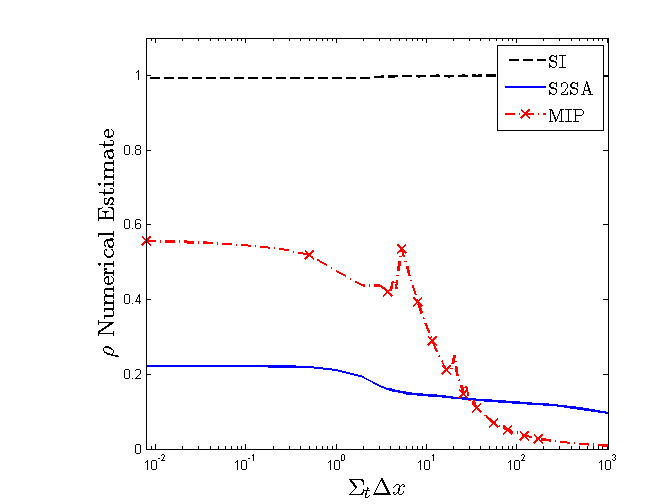
\includegraphics[width=10cm]{chapter4_acceleration/Constant_XS_SN8_P1_Gauss_Solvers.png}
\caption{Estimates of $\rho$ for different iterative techniques for $S_8$, $c=0.999$, linear SL Gauss.}
\label{fig:p1_gauss}
\end{figure}
In \fig{fig:p1_lobatto}, we compare the $\rho$ estimates of SI, S2SA, and MIP DSA for linear SL Lobatto differencing.  Results indicate that both S2SA and MIP DSA are compatible with SL Lobatto neutron transport.
MIP DSA for linear SL Lobatto exhibits the same peaking as observed with linear SL Gauss, though the peak is slightly smoother. 
\begin{figure}[!htp]
\centering
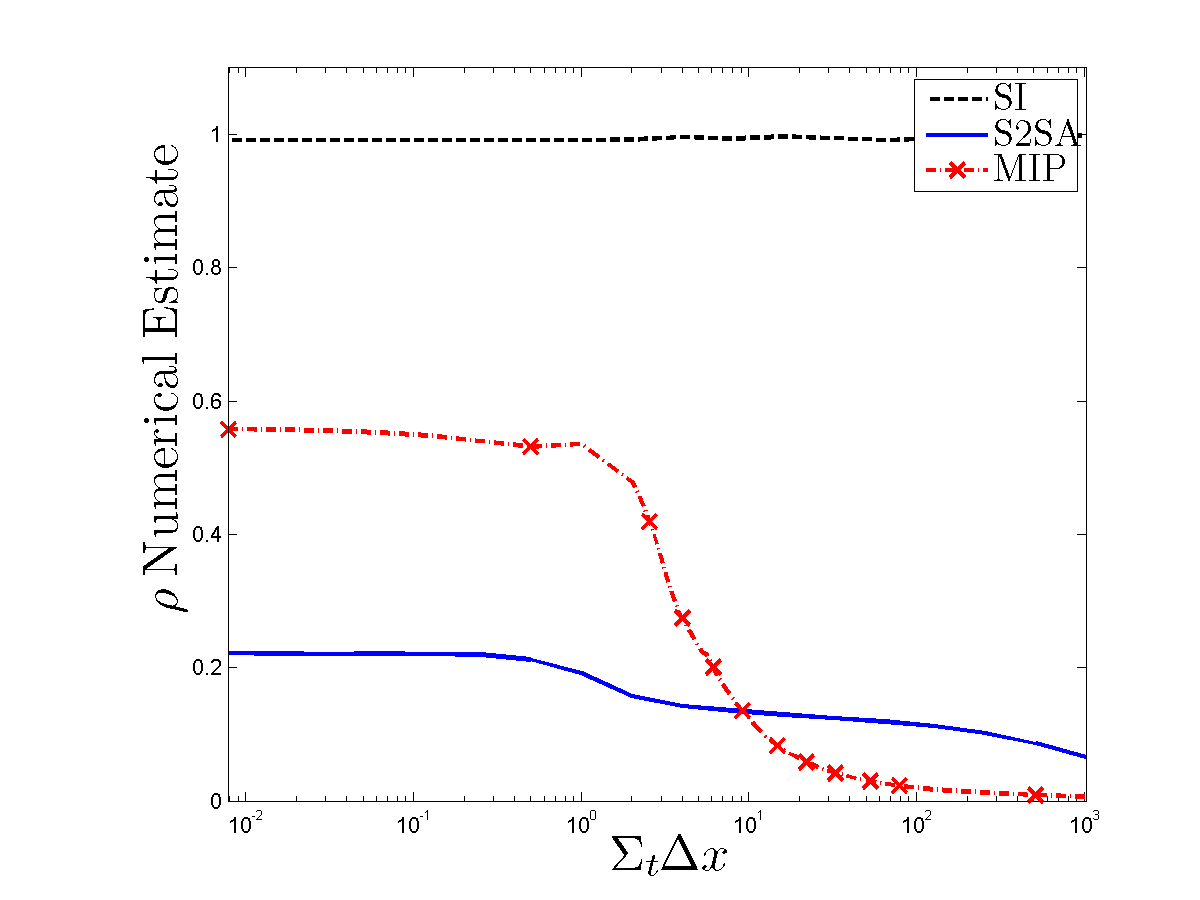
\includegraphics[width=10cm]{chapter4_acceleration/Constant_XS_SN8_P1_Lobatto_Solvers.png}
\caption{Estimates of $\rho$ for different iterative techniques for $S_8$, $c=0.999$, linear SL Lobatto.}
\label{fig:p1_lobatto}
\end{figure}
We now attempt to find a value of $c$ and the $S_N$ order that result in the worst (largest) value of $\rho$ for S2SA and MIP DSA. 
From \fig{fig:p1_gauss} and \fig{fig:p1_lobatto}, we expect that the choice of DFEM interpolation point will have nearly negligible effect on $\rho$, but continue to compare SL Lobatto and SL Gauss solutions to one another for completeness.

In \fig{fig:mip_gauss_as_fun_sn} and \fig{fig:mip_lobatto_as_fun_sn} we compare $\rho$ as a function of $S_N$ order, for linear SL Gauss and linear SL  Lobatto, respectively, with $c=0.999$.
\begin{figure}[!htp]
\centering
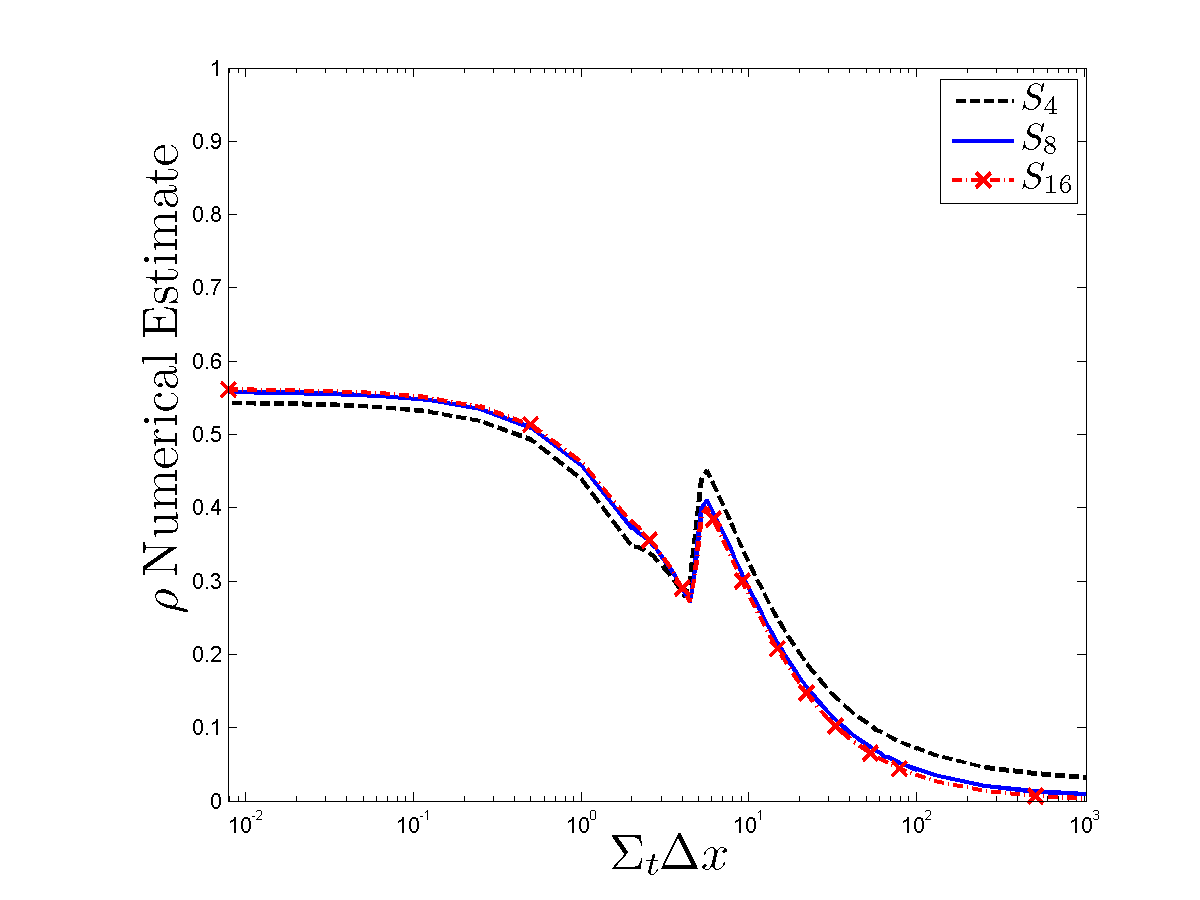
\includegraphics[width=10cm]{chapter4_acceleration/Constant_XS_sn_comparions_MIP_Gauss.png}
\caption{Estimates of $\rho$ for MIP DSA as a function of  $S_N$ order for $c=0.999$ cubic SL Lobatto.}
\label{fig:mip_gauss_as_fun_sn}
\end{figure}
%
%
\begin{figure}[!hbp]
\centering
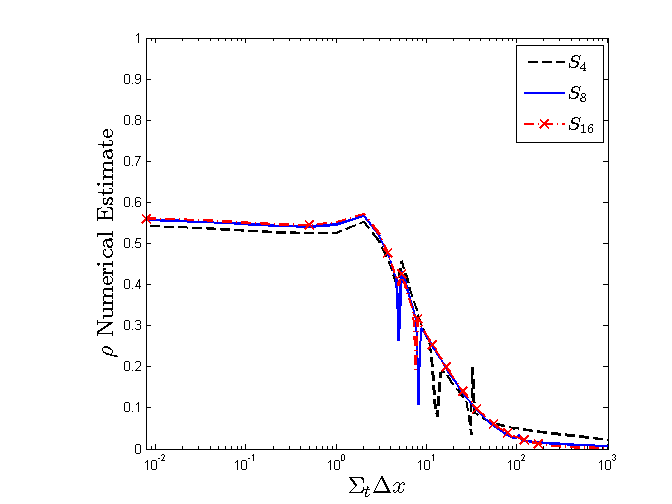
\includegraphics[width=10cm]{chapter4_acceleration/Constant_XS_sn_comparions_MIP_Lobatto.png}
\caption{Estimates of $\rho$ for MIP DSA as a function of  $S_N$ order for $c=0.999$ cubic SL Lobatto.}
\label{fig:mip_lobatto_as_fun_sn}
\end{figure}
%
%
Likewise, in \fig{fig:s2sa_gauss_as_fun_sn} and \fig{fig:s2sa_lobatto_as_fun_sn}, we compute $\rho$ for S2SA as a function of $S_N$ order for linear SL Gauss and linear SL Lobatto, respectively.
\begin{figure}[!htp]
\centering
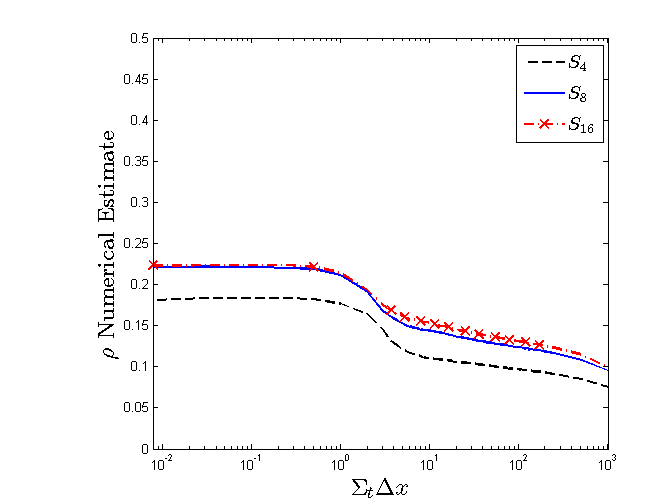
\includegraphics[width=10cm]{chapter4_acceleration/Constant_XS_sn_comparions_S2SA_Gauss.png}
\caption{Estimate of $\rho$ for S2SA as a function of $S_N$ order for $c=0.999$ for  cubic SL Lobatto.}
\label{fig:s2sa_gauss_as_fun_sn}
\end{figure}
%
%
\begin{figure}[!hbp]
\centering
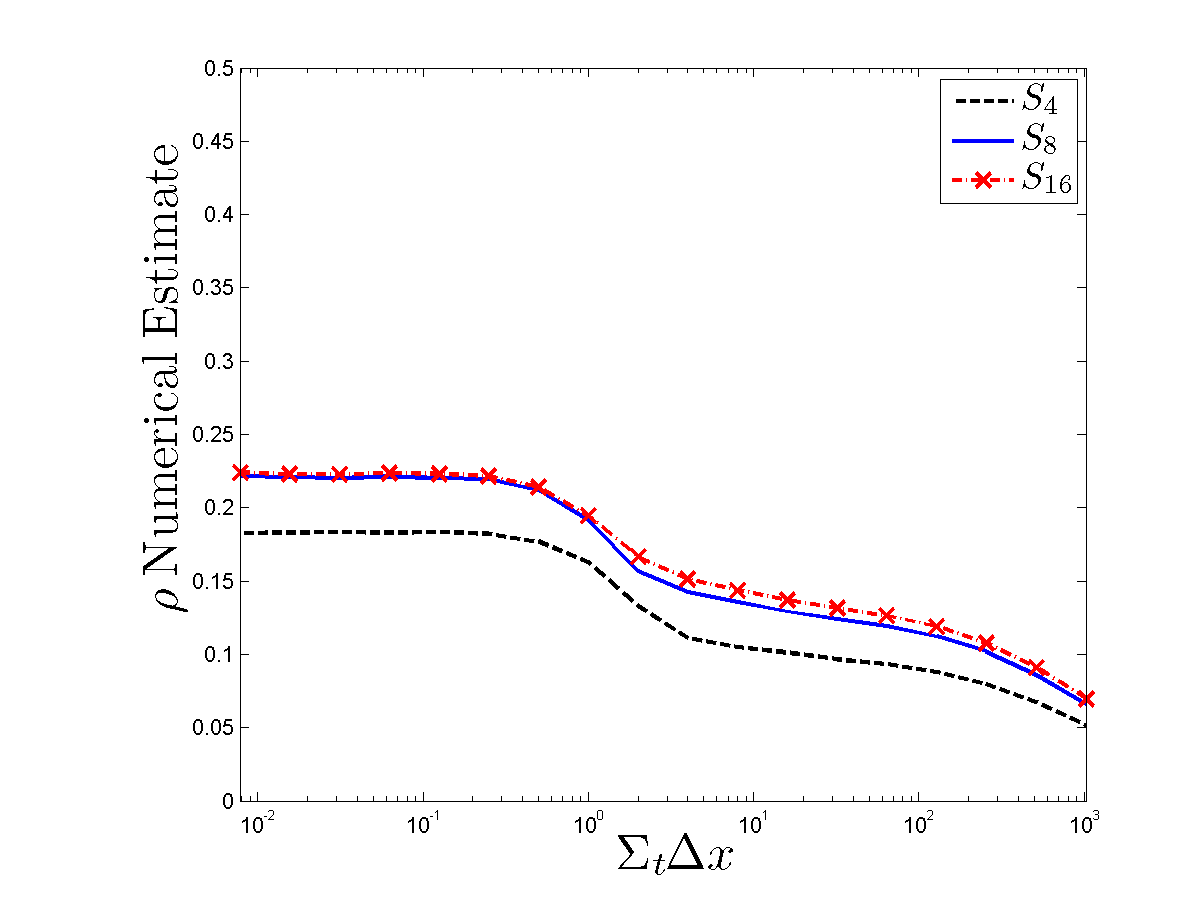
\includegraphics[width=10cm]{chapter4_acceleration/Constant_XS_sn_comparions_S2SA_Lobatto.png}
\caption{Estimate of $\rho$ for S2SA as a function of $S_N$ order for $c=0.999$ for  cubic SL Lobatto.}
\label{fig:s2sa_lobatto_as_fun_sn}
\end{figure}
Every figure in \figs{fig:mip_gauss_as_fun_sn}{fig:s2sa_lobatto_as_fun_sn}, indicates that the higher the $S_N$ order, the larger $\rho$. 
However, the value of $\rho$ obtained with $S_8$ is only slightly smaller than the $\rho$ of $S_{16}$, and as such we prefer the reduced computational work of $S_8$ simulations to $S_{16}$ in examining the iterative effectiveness of S2SA and MIP DSA for higher order DFEM.

Figure \ref{fig:mip_gauss_as_fun_c} and \fig{fig:mip_lobatto_as_fun_c} examine the effect of $c$ on $\rho$ for MIP DSA with the linear SL Gauss and SL Lobatto schemes.
The close $c$ is to unity, the larger the estimate of $\rho$, but we observe little increase in $\rho$ in moving from $c=0.999$ to $c=0.9999$, so we find that assuming $c=0.999$ is suficient for our purposes of determining the effectiveness of MIP DSA for higher order SL Lobatto.  Comparing our estimates of $\rho$ of S2SA, as a function of $c$, for linear SL Gauss and SL Lobatto in \fig{fig:s2sa_gauss_as_fun_c} and \fig{fig:s2sa_lobatto_as_fun_c}, respectively, we also conclude that the closer $c$ is to unity, the larger, $\rho$, but there is negligible increase from $c=0.999$ to $c=0.9999$.
\begin{figure}[!hbp]
\centering
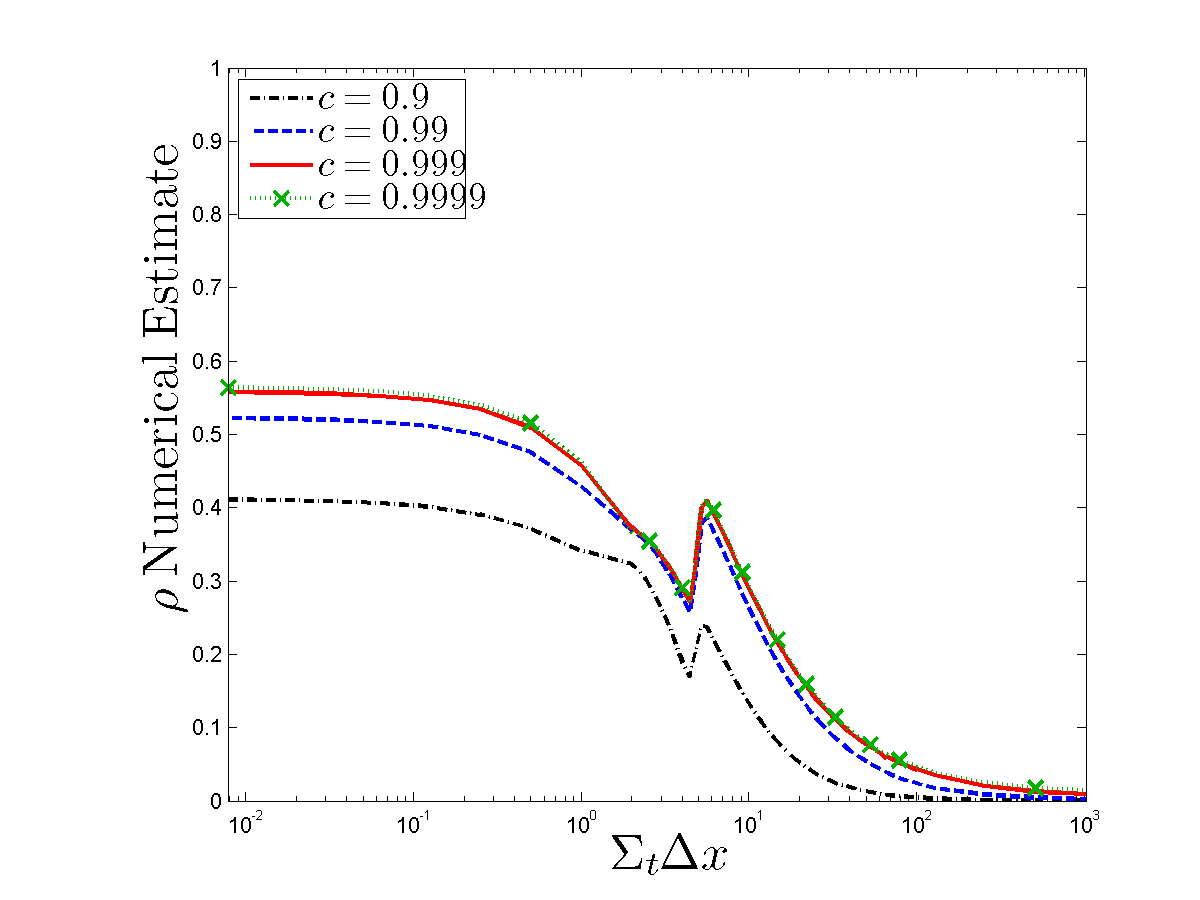
\includegraphics[width=10cm]{chapter4_acceleration/Constant_XS_c_comparions_MIP_Gauss.png}
\caption{Estimates of $\rho$ for MIP DSA as a function of $c$  for  $S_8$  cubic SL Lobatto.}
\label{fig:mip_gauss_as_fun_c}
\end{figure}
\vfill{}
\pagebreak
\begin{figure}[!htp]
\centering
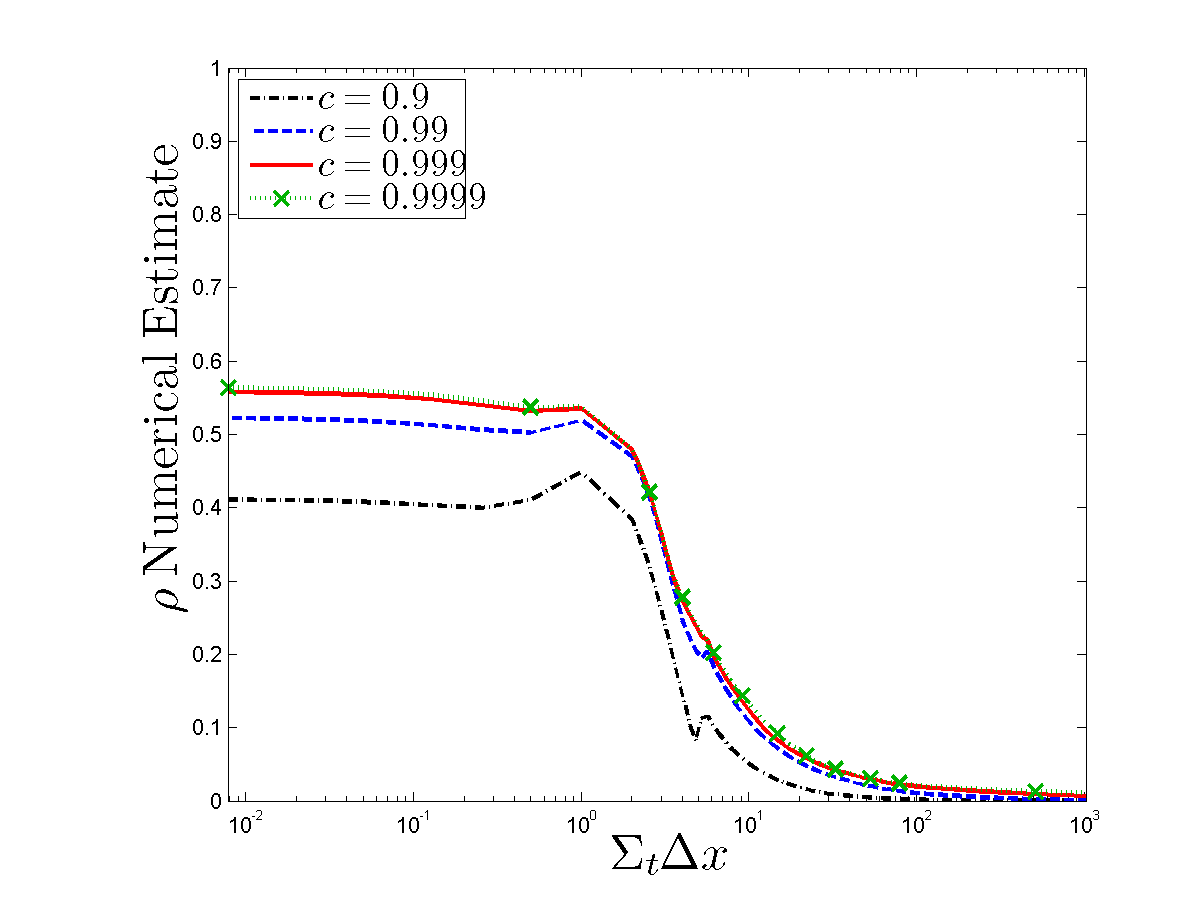
\includegraphics[width=10cm]{chapter4_acceleration/Constant_XS_c_comparions_MIP_Lobatto.png}
\caption{Estimates of $\rho$ for MIP DSA as a function of $c$  for  $S_8$  cubic SL Lobatto.}
\label{fig:mip_lobatto_as_fun_c}
\end{figure}
\begin{figure}[!hbp]
\centering
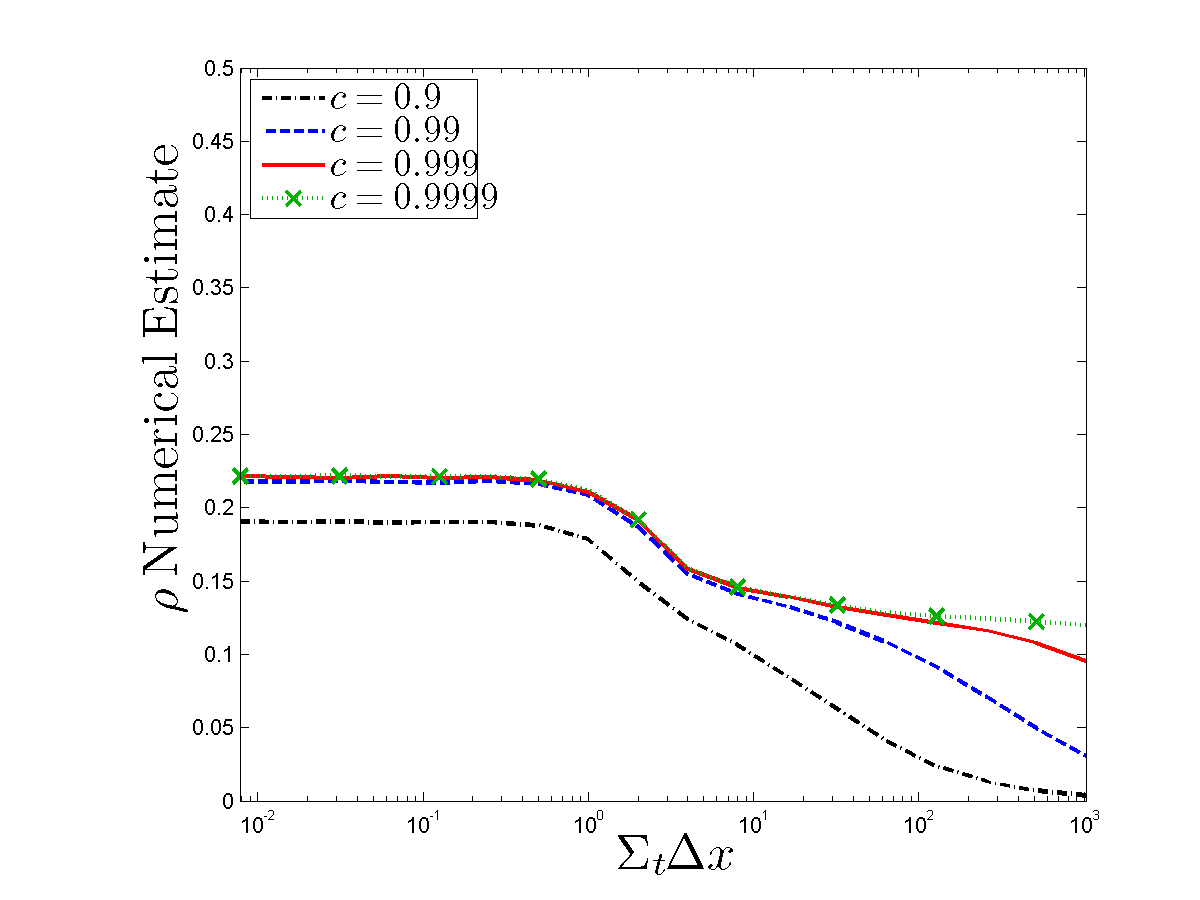
\includegraphics[width=10cm]{chapter4_acceleration/Constant_XS_c_comparions_S2SA_Gauss.png}
\caption{Estimates of $\rho$ for MIP DSA as a function of $c$  for  $S_8$  cubic SL Lobatto.}
\label{fig:s2sa_gauss_as_fun_c}
\end{figure}

%
%
\begin{figure}[!htp]
\centering
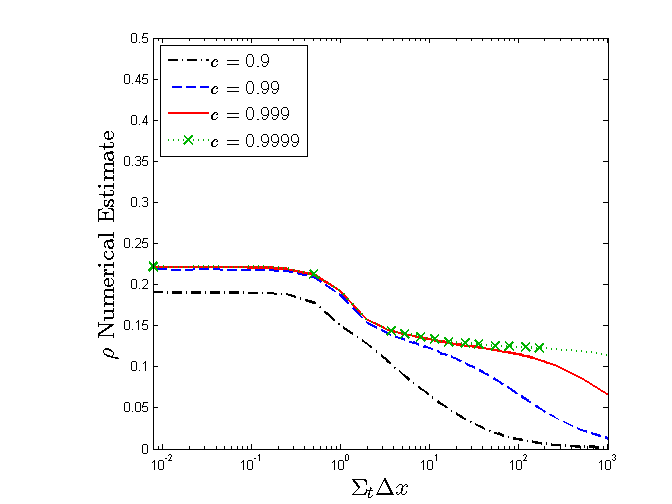
\includegraphics[width=10cm]{chapter4_acceleration/Constant_XS_c_comparions_S2SA_Lobatto.png}
\caption{Estimates of $\rho$ for MIP DSA as a function of $c$  for  $S_8$  cubic SL Lobatto.}
\label{fig:s2sa_lobatto_as_fun_c}
\end{figure}

Having determined that for linear DFEM, $c=0.999$ and $S_8$ will yield nearly maximal $\rho$, we calculate $\rho$ as a function of $P$ for MIP DSA acceleration of SL Gauss and SL Lobatto transport spatial discretizations in \fig{fig:mip_gauss} and \fig{fig:mip_lobatto}, respectively.  Figure \fig{fig:mip_gauss} confirms the results of \cite{mip_dsa}, and \fig{fig:mip_lobatto} indicates that so long as the MIP DSA operator is defined using the same numerical scheme (lumping technique and DFEM trial space) as the neutron transport spatial discretization, MIP DSA is an effective iterative acceleration technique.
Similarly, \fig{fig:s2sa_gauss} and \fig{fig:s2sa_lobatto} indicate that S2SA is an effective iterative acceleration technique for self-lumping higher order DFEM neutron transport spatial discretizations.
\vfill{}
\begin{figure}[!htp]
\centering
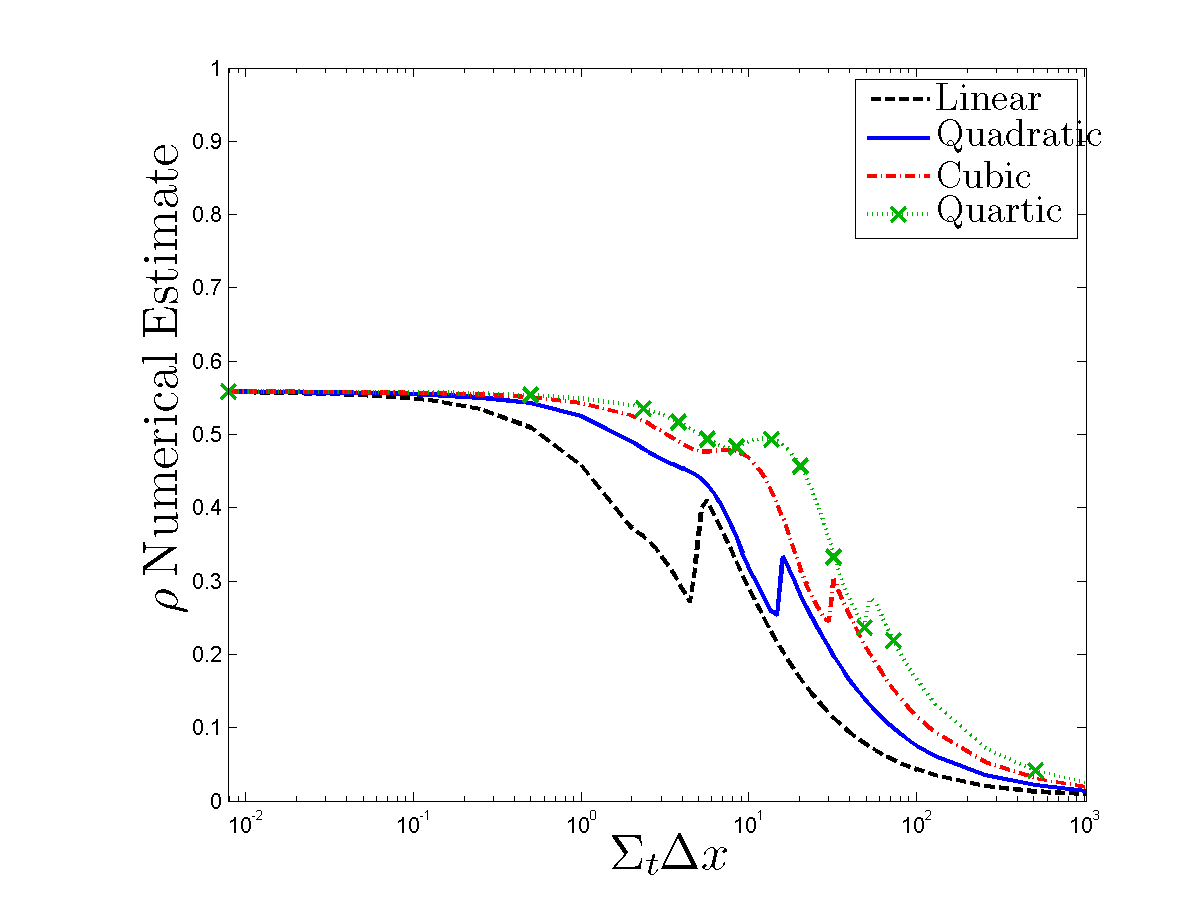
\includegraphics[width=10cm]{chapter4_acceleration/Constant_XS_SN8_MIP_Gauss.png}
\caption{Estimates of $\rho$ for MIP as a function of $S_8$, $c=0.999$, SL Gauss as a function of trial space degree.}
\label{fig:mip_gauss}
\end{figure}
%
%
\begin{figure}[!hbp]
\centering
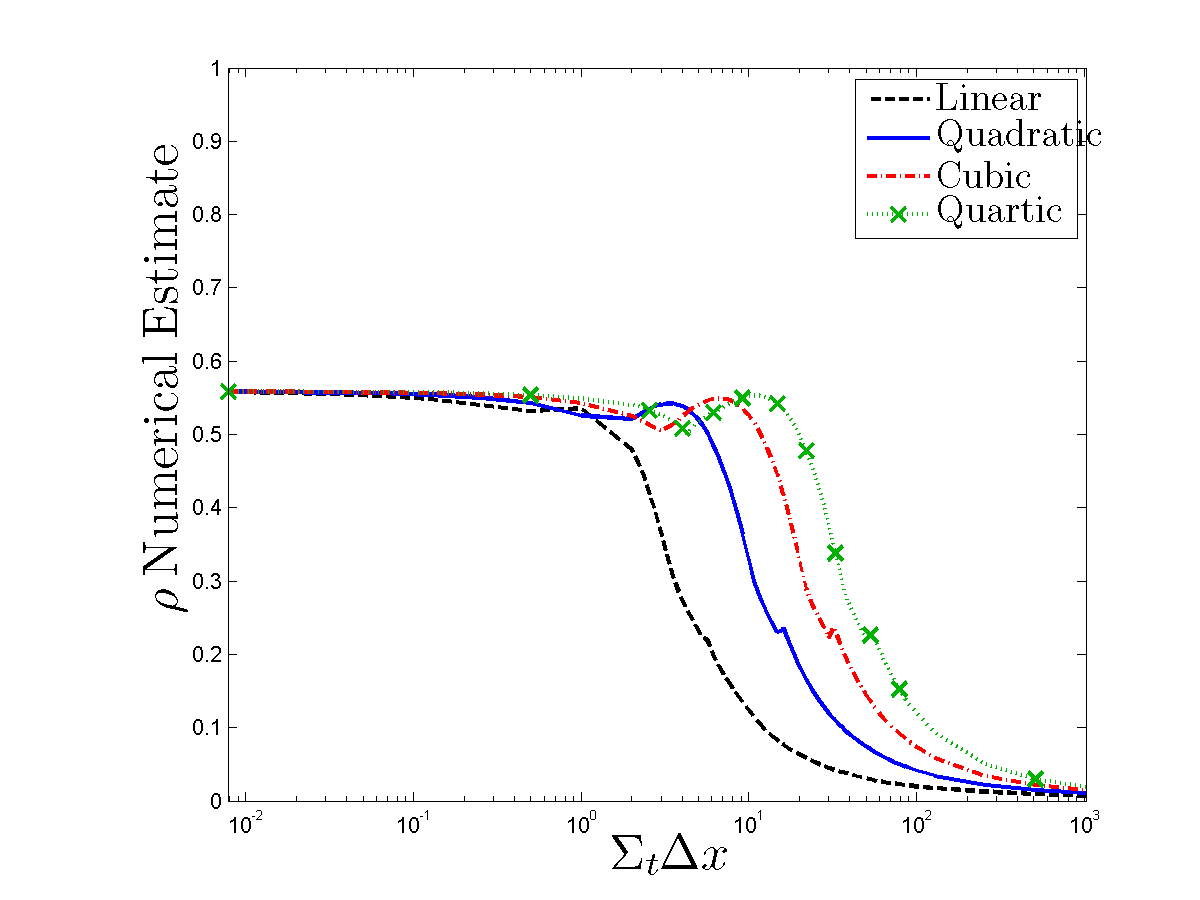
\includegraphics[width=10cm]{chapter4_acceleration/Constant_XS_SN8_MIP_Lobatto.png}
\caption{Estimates of $\rho$ for MIP DSA as a function of $S_8$, $c=0.999$, SL Lobatto as a function of trial space degree.}
\label{fig:mip_lobatto}
\end{figure}
%
%
\begin{figure}[!htp]
\centering
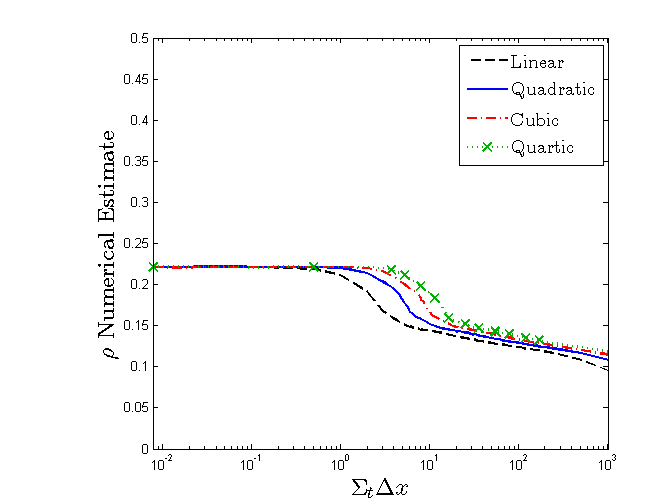
\includegraphics[width=10cm]{chapter4_acceleration/Constant_XS_SN8_S2SA_Gauss.png}
\caption{Estimates of $\rho$ for S2SA as a function of $S_8$, $c=0.999$, SL Gauss as a function of trial space degree.}
\label{fig:s2sa_gauss}
\end{figure}
%
%
\begin{figure}[!hbp]
\centering
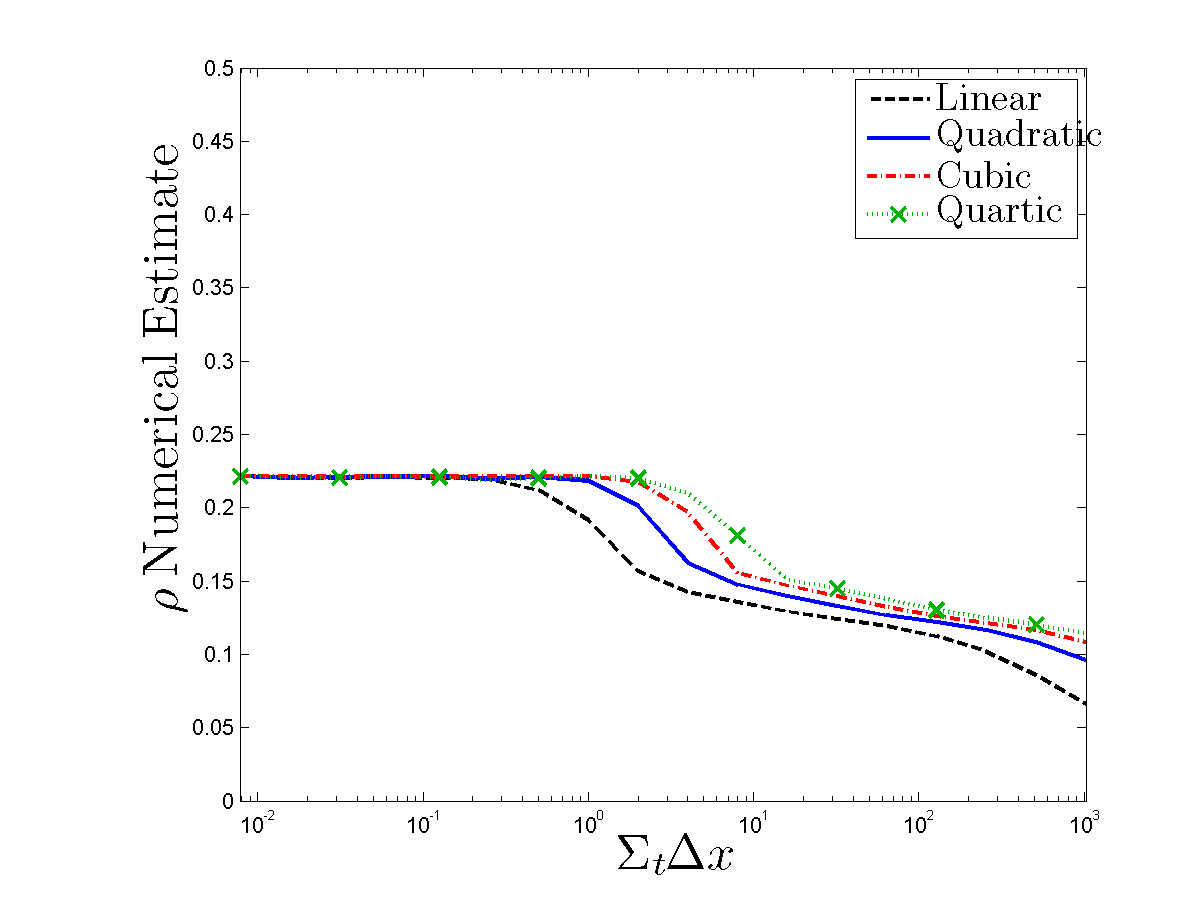
\includegraphics[width=10cm]{chapter4_acceleration/Constant_XS_SN8_S2SA_Lobatto.png}
\caption{Estimates of $\rho$ for S2SA as a function of $S_8$, $c=0.999$, SL Lobatto as a function of trial space degree.}
\label{fig:s2sa_lobatto}
\end{figure}
\pagebreak

\subsection{Spatially Varying Cross Section Scattering Problem}
\label{sec:chap4_variable_xs}

To test the effectiveness of MIP DSA and S2SA for a problem with a spatially varying cross section, we again consider a slab $x\in\left[0,20[cm] \right]$.
We impose 
\benum
\Sigma_t(x) = \Sigma_{t,0} \exp\left[ \frac{\abs{\left(10 -x  \right)}  }{2} \right] \pep
\eenum
We hold $c$ constant in space.
We will estimate $\rho$ as a function of $\overline{\Sigma_t \Delta x}$, the average optical thickness of each mesh cell.
For values of $\overline{\Sigma_t \Delta x} > 2$, we will use 10 mesh cells, and adjust $\Sigma_{t,0}$ to achieve the desired optical thickness.
For values of $\overline{\Sigma_t \Delta x} < 2$, we will hold $\Sigma_{t,0}$ constant, and increase the number of mesh cells.
We wish to maintain a total slab optical thickness of at least 20 mean free paths.  Since,
\begin{subequations}
\beanum
\text{Total Mean Free Path} &=& 2 \int_0^{10~cm}{\Sigma_{t,0} \exp\left[ \frac{10-x}{2} \right]~dx} \\
\text{Total Mean Free Path} &=& 4\Sigma_{t,0} \left( \exp[5] - 1 \right) \pec
\eeanum
the minimum value of $\Sigma_{t,0}$ is:
\benum
\Sigma_{t,0} = \frac{5}{  \exp[5] - 1  }\pep
\eenum
For values of $\overline{\Sigma_t \Delta x} > 2$,
\beanum
10 \overline{\Sigma_t \Delta x} &=& 4\Sigma_{t,0} \left( \exp[5] - 1 \right) \\
\Sigma_{t,0} &=& \frac{5\overline{\Sigma_t \Delta x}}{2 \left( \exp[5] - 1 \right) } \pep
\eeanum
\end{subequations}

